\documentclass{report}
\usepackage[utf8]{inputenc}
\usepackage[spanish]{babel}
\usepackage[margin=2cm]{geometry}
\usepackage{graphicx}
\usepackage{float}
\usepackage{titlesec}
\usepackage{caption}
\usepackage{listings}
\usepackage{xcolor}
\usepackage{array}
\usepackage{booktabs}
\usepackage{tabularx}
\usepackage{multirow}
\usepackage{amsmath}
\usepackage{hyperref}
\usepackage{ragged2e} 
\usepackage{lipsum}

\definecolor{codegreen}{rgb}{0,0.6,0}
\definecolor{codegray}{rgb}{0.5,0.5,0.5}
\definecolor{codepurple}{rgb}{0.58,0,0.82}
\definecolor{backcolor}{rgb}{0.95,0.95,0.95}

\lstset{
    basicstyle=\ttfamily,
    inputencoding=utf8,
    extendedchars=true,
    literate=%
    {á}{{\'a}}1
    {é}{{\'e}}1
    {í}{{\'i}}1
    {ó}{{\'o}}1
    {ú}{{\'u}}1
    {ñ}{{\~n}}1
    {Á}{{\'A}}1
    {É}{{\'E}}1
    {Í}{{\'I}}1
    {Ó}{{\'O}}1
    {Ú}{{\'U}}1
    {Ñ}{{\~N}}1
}

\lstdefinestyle{mystyle}{
    backgroundcolor=\color{backcolor},
    commentstyle=\color{codegreen},
    keywordstyle=\color{red},
    numberstyle=\tiny\color{codegray},
    stringstyle=\color{codepurple},
    basicstyle=\ttfamily\footnotesize,
    breakatwhitespace=false,
    breaklines=true,
    captionpos=b,
    keepspaces=true,
    numbers=left,
    showspaces=false,
    showstringspaces=false,
    showtabs=false,
    tabsize=2  
}

\titleformat{\section}
{\huge\bfseries}{\thesection.}{1em}{}
\titleformat{\subsection}
{\large\bfseries}{\thesubsection}{1em}{}

\renewcommand\thesection{\arabic{section}}

\title{\Huge{\textbf{Diseño Inicial del Sistema}}\\
\Large{\textbf{Ingeniería de Software Para Sistemas Intelgentes}}}
\author{Diego Castillo Reyes\\Marthon Leobardo Yañez Martinez\\Aldo Escamilla Resendiz}

\graphicspath{{imagenes/}}

\begin{document}
\maketitle
\section{Diseño Operativo}




\section{Diseño de Interfaces}
    % Agrega DisenioPreliminar.jpg
    \begin{figure}[H]
        \centering
        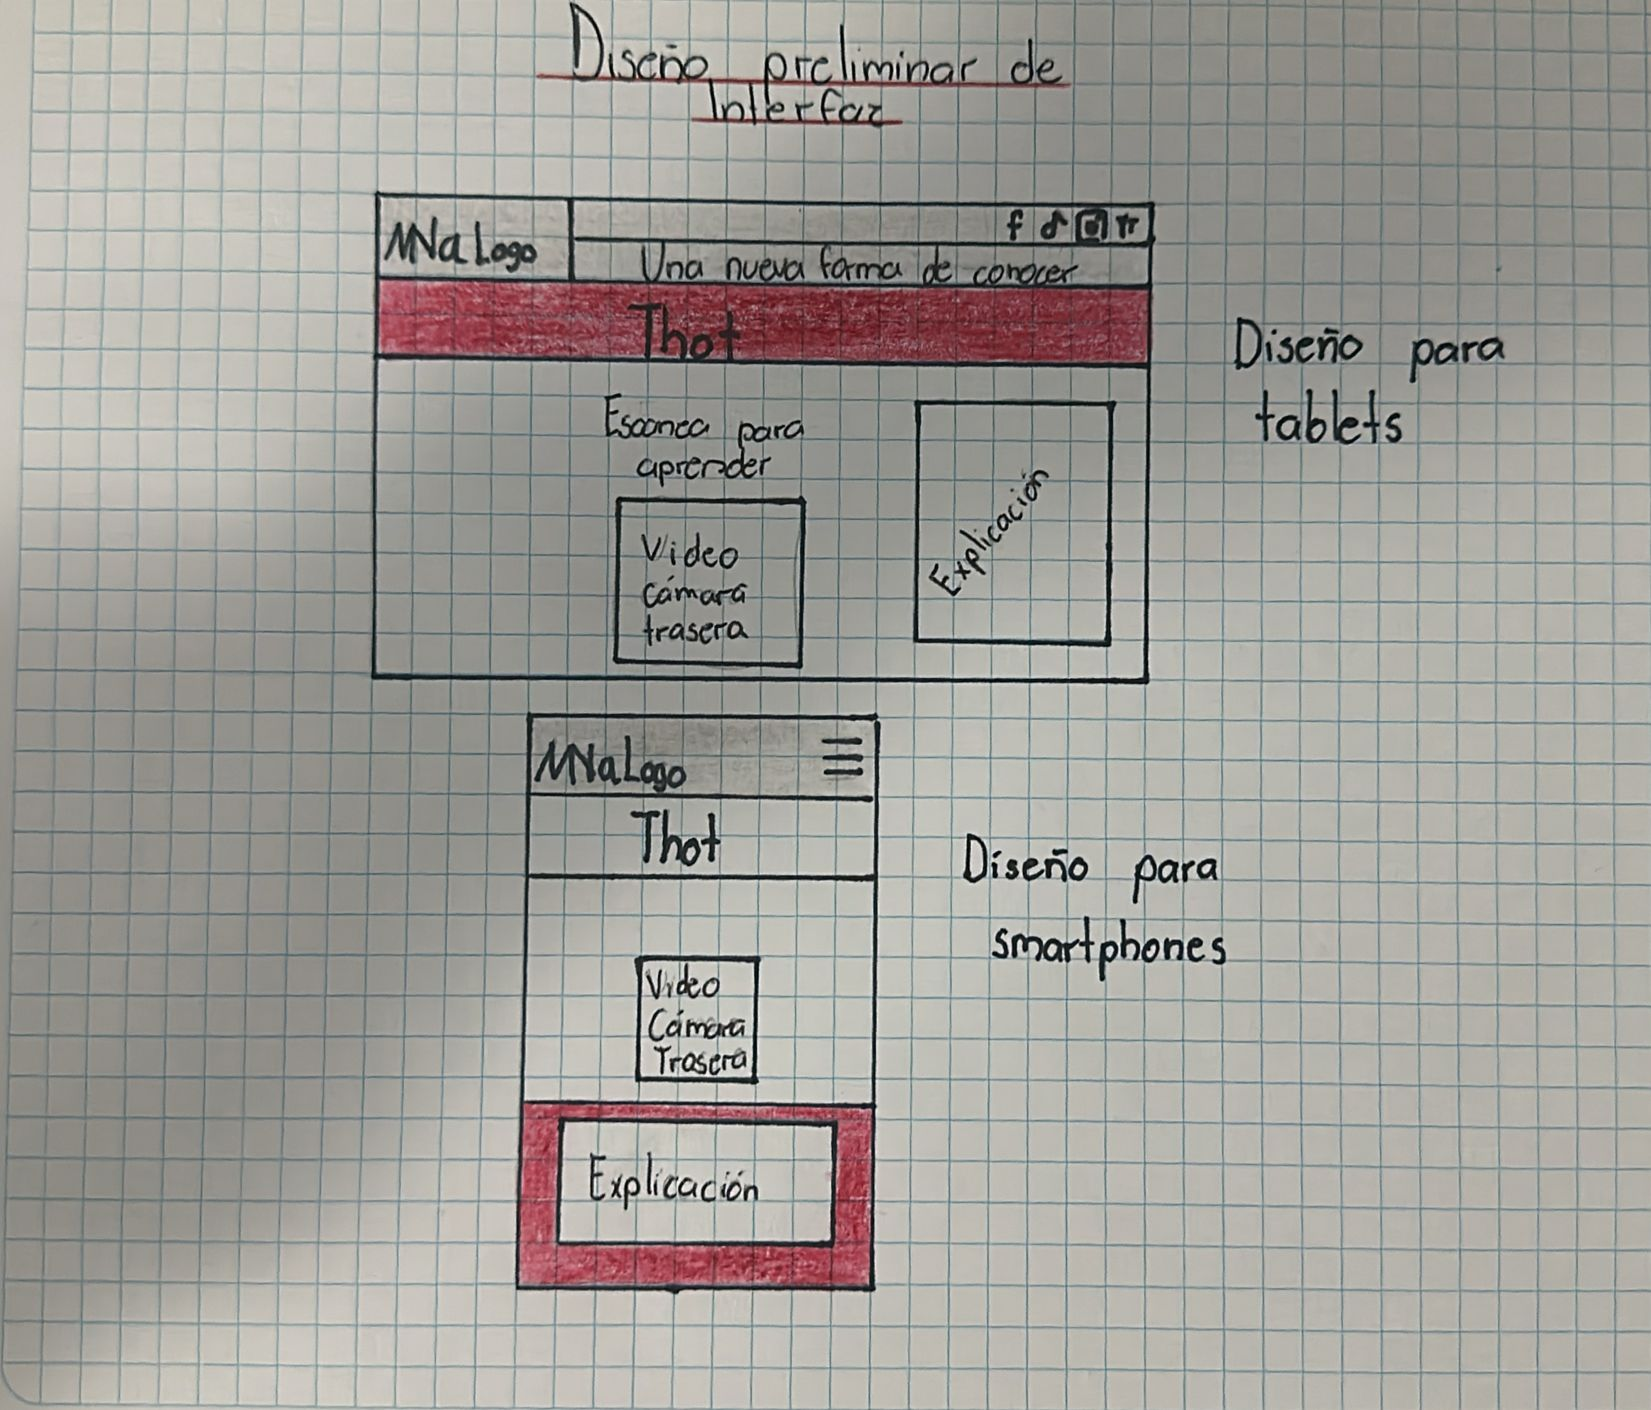
\includegraphics[width=0.8\textwidth]{DisenioPreliminar.jpeg}
        \caption{Diseño Preliminar de la Interfaz}
    \end{figure}
    En esta imagen se muestra el diseño preliminar de la interfaz de Thot donde se 
    contemplan dos tipos de dispositivos que usarían este software: los smartphones y las tablets
    debido a su movilidad y que la mayoría de personas llevarían de forma voluntaria al museo.
    
    \section{Expansion diagrama de procesos}

    \begin{figure}[H]
        \centering
        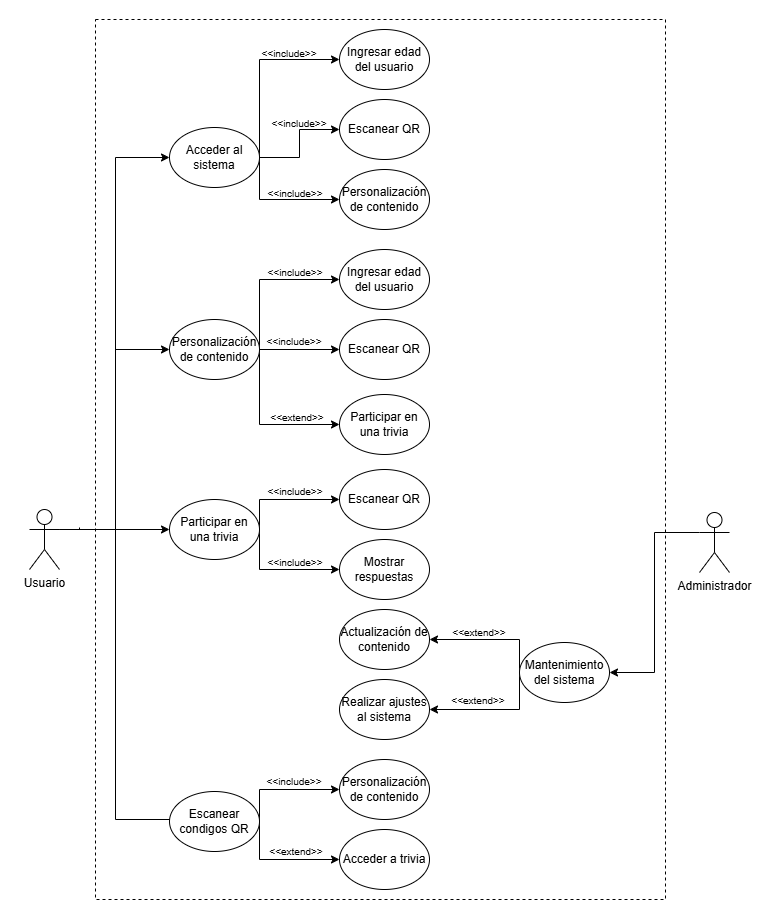
\includegraphics[width=0.8\textwidth]{Casos de uso.png}
        \caption{Expansion del Diagrama de Procesos}
    \end{figure}

    \subsection*{Caso de uso 1: Acceder al sistema}
    Un usuario accede al sistema desde un sitio web y lo utiliza para obtener información personalizada a través de códigos QR.
    
    \textbf{Actor:} Usuario.

    \textbf{Relaciones:}
    \begin{itemize}
        \item Include: Ingresar edad del usuario.\\
        Justificación: El ingreso de la edad es necesario para personalizar la experiencia antes de continuar con el acceso al sistema.
        \item Include: Escanear QR.\\
        Justificación: Escanear un QR es parte fundamental de este flujo, ya que permite acceder a la información.
        \item Include: Personalización de contenido.\\
        Justificación: La personalización de la información es clave para adecuar la experiencia del usuario.
    \end{itemize}

    \subsection*{Caso de uso 2: Personalización de contenido}
    El sistema personaliza la información y las trivias basadas en la edad del usuario.

    \textbf{Actor:} Usuario.

    \textbf{Relaciones:}
    \begin{itemize}
        \item Include: Ingresar edad del usuario.\\
        Justificación: La personalización depende directamente de la edad ingresada por el usuario.
        \item Include: Escanear QR.\\
        Justificación: El contenido se adapta con base en la información escaneada.
        \item Extend: Participar en una trivia.\\
        Justificación: La trivia es opcional, y este caso de uso se extiende solo si el usuario decide participar.
    \end{itemize}

    \subsection*{Caso de uso 3: Participar en una trivia}
    Los usuarios participan en una trivia después de haber escaneado varios códigos QR.

    \textbf{Actor:} Usuario.

    \textbf{Relaciones:}
    \begin{itemize}
        \item Include: Escanear QR.\\
        Justificación: Las preguntas de la trivia están basadas en los QR que el usuario ha escaneado, por lo que el escaneo es un paso necesario.
        \item Include: Mostrar respuestas con justificación.\\
        Justificación: Mostrar las respuestas correctas con justificación es parte del flujo normal después de completar la trivia.
    \end{itemize}

    \subsection*{Caso de uso 4: Mantenimiento del sistema}
    Un técnico realiza el mantenimiento regular del sistema cada 6 meses.

    \textbf{Actor:} Administrador.

    \textbf{Relaciones:}
    \begin{itemize}
        \item Extend: Actualización de contenido.\\
        Justificación: El administrador del sistema actualiza la base de datos con nueva información.
        \item Extend: Realizar ajustes al sistema.\\
        Justificación: Si se encuentran errores o fallas, se extiende el caso de uso para realizar las correcciones necesarias.
    \end{itemize}

    \subsection*{Caso de uso 5: Escanear códigos QR}
    Los usuarios escanean códigos QR ubicados en diferentes partes de la sala del museo para obtener información.

    \textbf{Actor:} Usuario.

    \textbf{Relaciones:}
    \begin{itemize}
        \item Include: Personalización de contenido.\\
        Justificación: La información obtenida por el QR se adapta automáticamente a la edad del usuario y otros parámetros.
        \item Extend: Acceder a trivia.\\
        Justificación: Después de escanear varios QR, el sistema puede extenderse para ofrecer al usuario la opción de participar en una trivia relacionada con la información que ha escaneado.
    \end{itemize}

\end{document}